\section{Constrained Directional Rigidity}
\label{sec:constrained_model}

\todoin{Update definitions to match formulation used here}
\todoin{Update notation used in this section}

\begin{figure}[t]
    \centering
    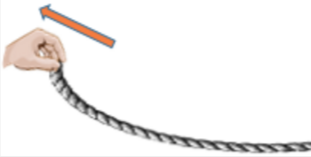
\includegraphics[width=.49\linewidth]{Intro_drag}\hfill
    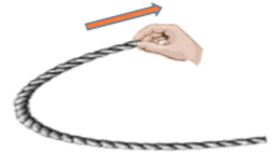
\includegraphics[width=.49\linewidth]{Intro_pull}%
    \caption{An illustrative example of directional rigidity. Left: The rope moves almost rigidly when dragging it by one end to the left. Right: The rope deforms when pulling it on the right in the opposite direction.}
    \label{fig:intro_directional_rigidity}
\end{figure}

While the diminishing rigidity Jacobian method has been used to do practical manipulation tasks with a deformable object with a precise physical model, we observe that this rigidity does not only diminish as the distance from the gripper increases. Instead, it is a function of a larger set of variables derived from the configuration of the object. The rigidity also depends on the direction of gripper motion. Fig.~\ref{fig:intro_directional_rigidity} shows an example of an object's \textit{directional rigidity}. In addition capturing the effects of directional rigidity, we seek to address contact with the environment, increasing the accuracy of $\tilde \DeformForwardFn$. 

\subsection{Geometric Model of Deformable Object Motion}

\subsubsection{Model Overview}
The approximate model locally describes the object's motion when given a motion of the grippers. Below we describe our approach first by specifying the model and then enforcing collision constraints on the prediction this model makes.

The current state of the deformable object is a function of the current gripper pose, the history of gripper motions that have been applied, the object's initial configuration, and the obstacles in the environment:

\begin{equation}
    \deformconfig = \DeformMappingExpanded
\end{equation}

To create a predictive model, we need to compute how $\deformconfig$ changes as a result of changing the gripper pose. Taking the time derivative of the above we obtain
\begin{equation}
\frac{d \deformconfig}{d t} = 
    \frac{\partial \DeformMapping}{\partial \gripperconfig}  \frac{\partial \gripperconfig}{\partial t} + 
    \frac{\partial \DeformMapping}{\partial \robotconfighist}\frac{\partial \robotconfighist}{\partial t} + 
    \frac{\partial \DeformMapping}{\partial \deformconfig_0} \frac{\partial \deformconfig_0}{\partial t} +
    \frac{\partial \DeformMapping}{\partial \obstacle}       \frac{\partial \obstacle}{\partial t}
\end{equation}

\todoin{Move this jacobian math definition up to the more generic math section.}
\noindent Only the first term is non-zero, thus
\begin{equation}
    \deformvel = \frac{\partial \DeformMappingExpanded}{\partial \gripperconfig} \grippervel
\end{equation}
$\frac{\partial \DeformMapping}{\partial \gripperconfig}$ is a matrix we call $\Jacobian$. In the previous section, $\Jacobian$ is assumed to be independent of $\grippervel$ and $\obstacle$, yielding\footnote{In this equation we replaced $\robotconfighist$ and $\deformconfig_0$ with $\deformconfig$, the current configuration of the object. $\robotconfighist$ and $\deformconfig_0$ are need in $\DeformMapping$ to compute the current state of the object, but if we can sense $\deformconfig$ directly (as we assume), then $\robotconfighist$ and $\deformconfig_0$ are not needed to compute $\tilde \Jacobian$.} $\frac{\partial \DeformMapping}{\partial \gripperconfig} = \Jacobian(\gripperconfig, \robotconfighist, \deformconfig_0) = \Jacobian(\gripperconfig, \deformconfig)$, which is analogous to a rigid-body Jacobian. While these assumptions allow a linear relationship between $\grippervel$ and $\deformvel$, and thus computational convenience, they are not accurate in many situations (see Figure \ref{fig:intro_directional_rigidity} for an example). In this section we change the definition of $\Jacobian$ to the following:

\begin{equation}
    \deformvel = \JacobianFull \grippervel = \DeformForwardFnFull
\end{equation}

We now describe how $\tilde \Jacobian$ is approximated, focusing on how it accounts for directional rigidity (using $\grippervel$) and how it enforces obstacle penetration constraints (using $\obstacle$).


\subsubsection{Directional Rigidity}
\todoin{Move parts that related to both diminishing rigidity and directional rigidity up a section}
\todoin{Go through and tie back to previous section}

We build on the idea proposed by Berenson~\cite{Berenson2013}, which approximates $\Jacobian$ based on the observation that the deformable object behaves rigidly near points grasped by the robot grippers. \cite{Berenson2013} encoded this effect through a simple function that only considered the distance of a point from the the nearest gripper. However, we find that we can exploit geometric information in the object's configuration to better predict the object's motion when we use a more complex model. We have observed that the key features of the deformable object configuration for predicting its motion are its deformability (which is determined by its material properties) and where it is slack. The deformation influences the transmission of the force from the grippers, i.e. the more stretchable the object, the more it will stretch when force is applied. However, when a region of the object is taut, regardless of how stretchable it is, it will move as if it were rigidly connected to a gripper (e.g. imagine a rope held taut by two grippers). We also must take into account that points are not influenced equally by different grippers, i.e. grippers farther away contribute less to the motion of a point than those closer to it.

\begin{figure}[t]
    \centering
    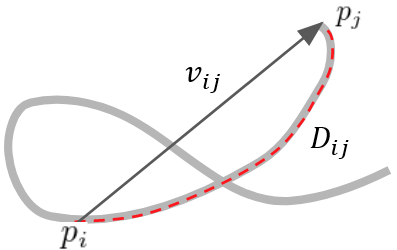
\includegraphics[width=1.5in]{method_geodesic.png}
    \caption{The length of the the red segment on the rope is the geodesic distance $\geodistIJ$. $\straightvecIJ$ is the vector showing the relative position of $\deformconfigJ$ with respect to $\deformconfigI$.}
    \label{fig:distance_vec_defs}
\end{figure}

To incorporate the above effects into our model, we define the following variables, which can be derived from $\gripperconfig, \grippervel$, and $\deformconfig$:
\begin{itemize}
    \item $\geodistIJ$: the geodesic distance (a scalar) between points $\deformconfigI$ and $\deformconfigJ$ on the surface of the object.
    \item $\straightvecIJ$: the vector starting at a point $\deformconfigI$ and ending at the point $\deformconfigJ$, as shown in Fig.~\ref{fig:distance_vec_defs}.
    \item $\gripperconfigG$: the configuration of gripper $\gripperidx$.
    \item $\grippervelG$: the velocity of gripper $\gripperidx$.
\end{itemize}

Furthermore, let $\closestpointIG$ be the index of the point with the minimal geodesic distance to $\deformconfigI$ among the ones grasped by the $\gripperidx$'th gripper. We address the notion of rigidity in object motion by considering the slackness of the object and reformulating the rigidity as a function of $\geodistIG$, $\straightvecIG$, and $\grippervelG$. For each point $\deformidx$ and gripper $\gripperidx$ we compute
\begin{equation}
\begin{split}
    \tilde \Jacobian(\deformidx, \gripperidx) 
                        &= \influenceIG \begin{bmatrix} \rigiditytransIG \JtransIG & \rigidityrotIG \JrotIG \end{bmatrix} \\
    \rigiditytransIG    &= \rigiditytrans(\geodistIG, \straightvecIG, \grippervelG) \\
    \rigidityrotIG      &= \rigidityrot(\geodistIG) \\
\end{split}
\label{eq:trans_rot_rigidity_diminishing_jacobian}
\end{equation}
$\rigiditytrans$ and $\rigidityrot$ are the corresponding translational and rotational diminishing rigidity factors defined by $\deformconfigI$ and gripper $\gripperidx$ (discussed below). 

Our goal is to encode the directional rigidity of the object motion into $\rigiditytrans$ and $\rigidityrot$ and use $\influenceIG$ to describe the \textit{influence} of gripper $\gripperidx$ on $\deformconfigI$. Intuitively, $\rigiditytrans$ should decrease with the increasing geodesic $\geodistIG$ distance between $\deformconfigI$ and $\deformconfig_{\closestpointIG}$. This is because the deformation of the region between $\deformconfigI$ and $\deformconfig_{\closestpointIG}$ will attenuate the transmitted force of the gripper's motion unless the object is taut. Since the effects on $\rigidityrotIG$ from $\grippervelG$ and $\straightvecIG$ are not as clear or significant as $\geodistIG$, we keep $\rigidityrotIG$ as a function of $\geodistIG$, where 
\begin{enumerate}
    \item $\rigidityrotIG$ ranges between $0$ and $1$.
    \item $\rigidityrotIG$ decreases as $\geodistIG$ increases.
\end{enumerate}
We give the definition of $\rigidityrotIG$ below.

From observation, we find two key reasons related to the slackness of the object that induce the diminishing rigidity effect for translation motion, and we aim to encode these factors into $\rigiditytransIG$. The first case is that the moving direction of $\grippervelG$ makes the region on the object between $\deformconfigI$ and $\deformconfig_{\closestpointIG}$ less taut. The second case is that this region is already slack. $\rigiditytransIG$ is thus a product of two terms:
\begin{equation}
    \rigiditytransIG = \tensionIG \slackIG
    \label{eq:Combined_directional_rigidity}
\end{equation}
where $\tensionIG$ addresses the effect in the first case (motion reducing tension), and $\slackIG$ addresses the effect in the second case (object slackness). Both $\tensionIG$ and $\slackIG$ are functions of some of $\gripperconfigG, \grippervelG, \deformconfigI$, or variables derived from these.

For $\deformconfigI$ on the object, we find $\tensionIG$ is greatly impacted by $\straightvecIG$ and $\transvelG$. Decomposing $\transvelG$ into $\transvelGRad$, the component in the direction of $\straightvecIG$, and $\transvelGPerp$, the component perpendicular to $\straightvecIG$. We observed that if $\transvelGRad$ is in the opposite direction to $\straightvecIG$, then it is more likely to make the intervening region slacker and thus reduce the transmission of force from the gripper to $\deformconfigI$. Moreover, if $\transvelGRad$ and $\straightvecIG$ are in the same direction when the object is not already slack, $\deformconfigI$ can move almost rigidly with $\grippervelG$. Fig.~\ref{fig:intro_directional_rigidity} shows an example of the impact of this alignment. Based on these observations, we design the function $\tensionIG = \tensionIGfull$ with the following properties:
\begin{enumerate}
    \item $\tensionIGfull$ ranges between $0$ and $1$.
    \item $\tensionIGfull > \tensionJGfull$
        \textbf{if} $\innerprod{\straightvecIG}{\transvelG} > \innerprod{\straightvecJG}{\transvelG}$
        \textbf{and} $\geodistIG = \geodistJG$.
    \item $\tensionIGfull > \tensionJGfull$
        \textbf{if} $\innerprod{\straightvecIG}{\transvelG} = \innerprod{\straightvecJG}{\transvelG}$
        \textbf{and} $\geodistIG > \geodistJG$.
\end{enumerate}
We give the definition of $\tensionIGfull$ below.


As mentioned above, $\slackIG$ depends on the current slackness of the intervening region. Without other external forces applied on the object, the pulling force applied by the robot will tend to unwind or unfold the object eventually (we do not consider cases where the object is tied into knots). For this reason,  the part of the intervening region on the object that is not already spread out is less likely to move rigidly with gripper $\gripperidx$. One indicator that can address this property is the ratio between the Euclidean distance between $\deformconfigI$ and $\deformconfig_{\closestpointIG}$, and the geodesic distance $\geodistIG$ between them. We denote $\distratioIG = \frac{||\straightvecIG||}{\geodistIG}$ to be this ratio. A larger $\distratioIG$ indicates a tauter intervening region. A tauter intervening region is more likely to result in $\deformvelI$ moving more rigidly. Thus we can design the function $\slackIG = \slackIGfull$ with the following properties:
\begin{enumerate}
    \item $\slackIGfull$ ranges between $0$ and $1$.
    \item $\slackIGfull = 1$ if $\distratioIG = 1$.
    \item $\slackIGfull > \slackJGfull$ if $\distratioIG > \distratioJG$
\end{enumerate}

Finally, $\influenceIG$, which captures the influence of gripper $\gripperidx$ on $\deformconfigI$ should have the following property (where $k$ is the index of a different gripper on the robot):
\begin{enumerate}
    \item $\influenceIG$ ranges between $0$ and $1$.
    \item $\influenceIG < \influenceIK$ if $\geodistIG > \geodistIK$.
    \item $\sum_{m = 1}^{\ngrippers} \influenceIM = 1$.
\end{enumerate}

\todo{Confirm that $\influenceIG$ has these properties.}


Through experimentation, we obtained good results with the following functions:
\begin{equation}
\begin{split}
    \tensionIGfull  &= e^{\drkdir \geodistIG \left(\cos \angle \left( \straightvecIG, \transvelG \right) - 1\right)} \\
    \slackIGfull    &= \left( \frac{\| \straightvecIG \|}{\geodistIG} \right) ^{\drkdist} \\
    \rigidityrotIG  &= e^{-\drkrot \geodistIG} \\
    \influenceIG    &= \frac{x_\gripperidx}{\sum_{m = 0}^\ngrippers x_m}\\
    x_m             &= \frac{\textrm{min} \{\geodistI{1}, \dots , \geodistI{\ngrippers}\}}{\geodist_m} 
\end{split}
\label{eq:directional_rigidity_factors}
\end{equation}
where $\drkdir$, $\drkdist$, and $\drkrot$ are non-negative parameters. Specifically, a larger $\drkdir$ indicates a greater impact on the diminishing in the rigidity from the motion reducing tension. A larger $\drkdist$ indicates a greater impact on the diminishing in the rigidity from the slackness of the object in the current state. A larger $\drkrot$ indicates a faster decrease in rotational rigidity as the distance from $\deformconfigI$ to the gripper increases. 
\todo{Confirm no negative before $\drkdir$ in Eq.~\eqref{eq:directional_rigidity_factors}}


\begin{figure}
    \centering
    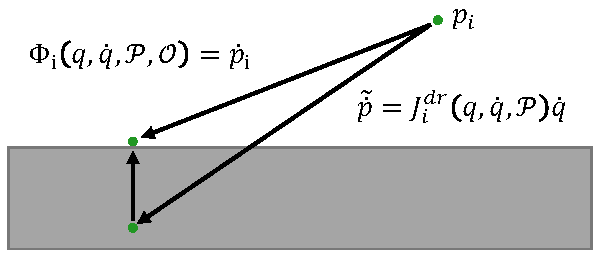
\includegraphics[width=3in]{point_projection}
    \caption{Projection process for points that are predicted to be in collision after movement.}
    \label{fig:point_projection}
\end{figure}

\subsubsection{Obstacle Penetration Constraints}

By combining the contributions of each individual gripper using the model developed above, we get a prediction of a point's movement from
\begin{equation}
    \approxPVI = \begin{bmatrix}
        \Jacobian(\deformidx, 1) & \dots & 
        \Jacobian(\deformidx, \ngrippers)
    \end{bmatrix} \grippervel = \Jacobian_{\deformidx}(\gripperconfig, \grippervel, \deformconfig) \grippervel
\end{equation}
However, at this stage, we haven't take into account the effect from the obstacles $\obstacle$. Thus the predicted $\approxPVI$ can move $\deformconfigI$ into an obstacle.

When the prediction of $\deformconfigI$ enters the obstacle, we project any penetration by the predicted $\approxPVI$ into the tangent space of the obstacle surface (Fig.~\ref{fig:point_projection}). Let $d_\deformidx < \| \approxPVI \|$ be the distance to collision in direction $\approxPVI$ from point $\deformconfigI$; let $\lambda_\deformidx = \frac{d_\deformidx}{\| \approxPVI \|}$; let $n_\deformidx$ be the unit surface normal of the obstacle in contact; and let $N_\deformidx = (\eye_{3\times 3} - \vec{n}_\deformidx \vec{n}_\deformidx^+)$. Then to account for obstacles we compute
\begin{equation}
    \tilde \Jacobian_\deformidx(\gripperconfig, \grippervel, \deformconfig, \obstacle) =
    \begin{cases}
        (\lambda_\deformidx + (1 - \lambda_\deformidx)N_\deformidx) \Jacobian_\deformidx(\gripperconfig, \grippervel, \deformconfig) & \text{if $\deformconfigI + \approxPVI$ in collision} \\
        \Jacobian_\deformidx(\gripperconfig, \grippervel, \deformconfig) & \text{otherwise}
    \end{cases}
\end{equation}
To generate $\Jacobian$ for all the points and grippers we compute $\Jacobian_\deformidx(\gripperconfig, \grippervel, \deformconfig)$ for each $\deformconfigI$. These matrices are modified using penetration constraints to get $\Jacobian_\deformidx(\gripperconfig, \grippervel, \deformconfig, \obstacle)$. These matrices are then stacked to obtain $\Jacobian(\gripperconfig, \grippervel, \deformconfig, \obstacle)$. Finally, we arrive at our approximate model: $\DeformForwardFnFull = \JacobianFull \grippervel$.